\begin{frame}
  \frametitle{Full Grid Discretization}
  \topline
  \vspace{-10px}
  \begin{block}{1. Function to discretize}
    \begin{figure}[!htp]

      \setbeamertemplate{caption}{\raggedright\insertcaption\par}
      \setbeamerfont{caption}{size=\footnotesize}
      \centering
      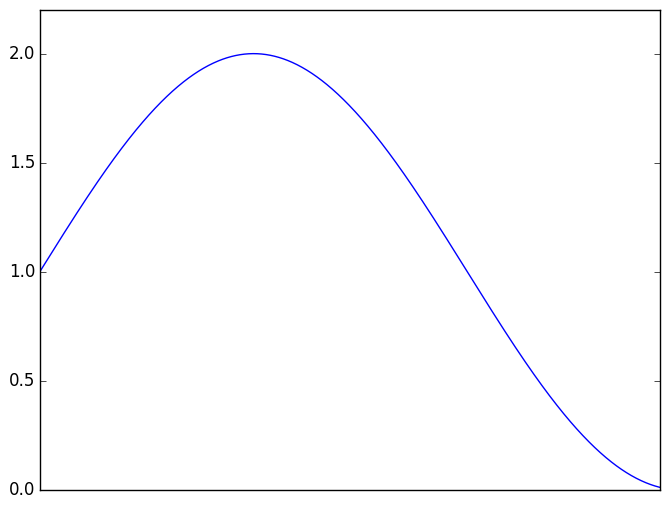
\includegraphics[width=7.5cm]{images/singlebasis_1}
      \vspace{-12px}
      \caption{$f(x) = 1 + \text{sin}(1.45\pi \cdot x)$}
    \end{figure}
  \end{block}
\end{frame}

\begin{frame}
  \frametitle{Full Grid Discretization}
  \topline
  \vspace{-10px}
  \begin{block}{2. Full, regular grid}
    \begin{figure}[!htp]

      \setbeamertemplate{caption}{\raggedright\insertcaption\par}
      \setbeamerfont{caption}{size=\footnotesize}
      \centering
      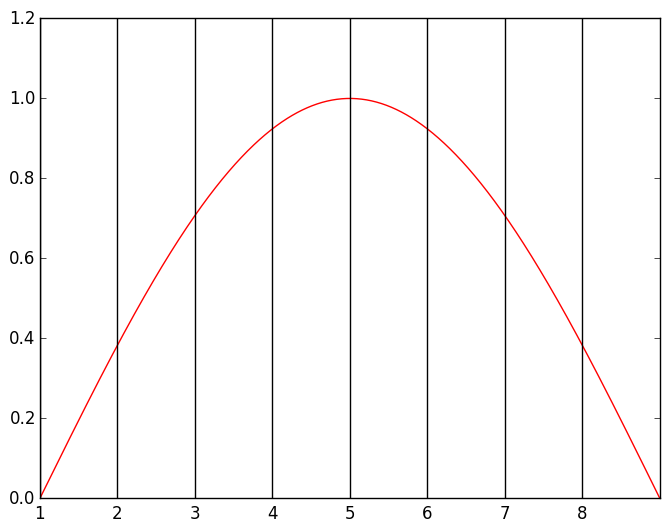
\includegraphics[width=7.5cm]{images/singlebasis_2}
      \vspace{-12px}
      \caption{Eight centered gridpoints $i \in \{1..8\}$}
    \end{figure}
  \end{block}
\end{frame}

\begin{frame}
  \frametitle{Full Grid Discretization}
  \topline
  \vspace{-10px}
  \begin{block}{3. Basis function (standard hat function)}
    \begin{figure}[!htp]

      \setbeamertemplate{caption}{\raggedright\insertcaption\par}
      \setbeamerfont{caption}{size=\footnotesize}
      \centering
      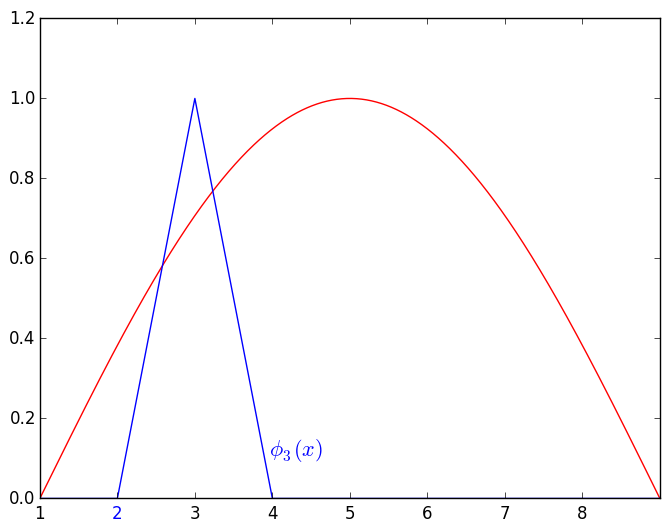
\includegraphics[width=7.5cm]{images/singlebasis_3}
      \vspace{-12px}
      \caption{$\phi(x - 2)$ with $\phi(x) = \text{max}(abs(1 - x), 0)$}
    \end{figure}
  \end{block}
\end{frame}

\begin{frame}
  \frametitle{Full Grid Discretization}
  \topline
  \vspace{-10px}
  \begin{block}{4. Coefficient $\alpha$ (Surplus)}
    \begin{figure}[!htp]

      \setbeamertemplate{caption}{\raggedright\insertcaption\par}
      \setbeamerfont{caption}{size=\footnotesize}
      \centering
      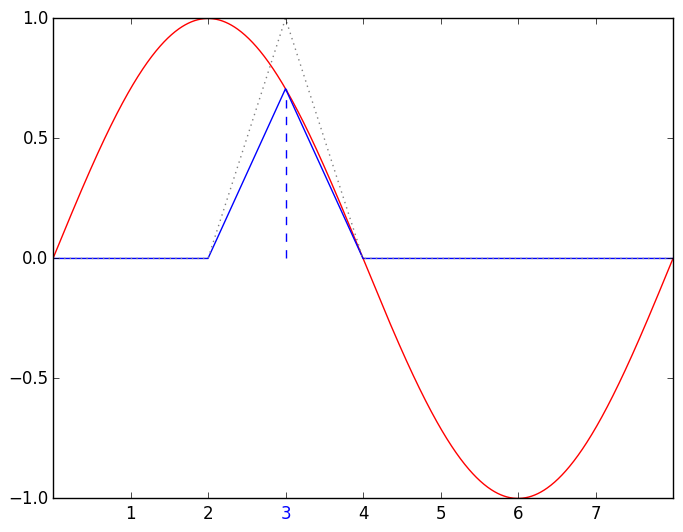
\includegraphics[width=7.5cm]{images/singlebasis_4}
      \vspace{-12px}
      \caption{$\alpha_3 \cdot \phi_3(x)$}
    \end{figure}
  \end{block}
\end{frame}

\begin{frame}
  \frametitle{Full Grid Discretization}
  \topline
  \vspace{-10px}
  \begin{block}{Sum over all basis functions}
    \begin{figure}[!htp]

      \setbeamertemplate{caption}{\raggedright\insertcaption\par}
      \setbeamerfont{caption}{size=\footnotesize}
      \centering
      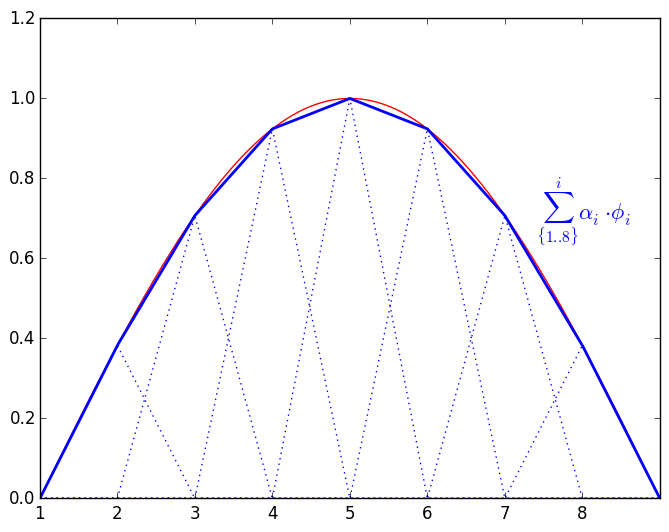
\includegraphics[width=7.5cm]{images/singlebasis_5}
      \vspace{-12px}
      \caption{$f(x) \approx \hat{f}(x) = \sum_i{\alpha_i \phi_i}$}
    \end{figure}
  \end{block}
\end{frame}

\begin{frame}
  \frametitle{Full Grid Discretization}
  \topline
  \vspace{-10px}
  \begin{block}{Full grid discretization in one dimension}
    \setbeamertemplate{enumerate items}[default]
    \begin{enumerate}
    \item A function $f(x)$ to discretize
    \item Gridpoints indexed by $i \in \{1,2,\dots\}$
    \item Basis/Ansatz functions; i.e. hat function $\phi(x)=\text{max}(1 - |x|, 0)$
    \item Coefficients $\alpha_i$ (Surplusses)
    \end{enumerate}
    \vspace{10px}
    \begin{center}
      $f(x) \approx$ $\hat{f}(x) = \sum_{i}^{}{\alpha_i \phi_i(x)}$
    \end{center}
  \end{block}
\end{frame}

\begin{frame}
  \frametitle{Full Grid Discretization}
  \topline
  \vspace{-10px}
  \begin{block}{Level of detail}
    \begin{itemize}
    \item Level $l \in \{1,2,4,8\dots\}$ defining the number of gridpoints $i$
    \end{itemize}
  \end{block}
  \begin{block}{$d > 1$ dimensions}
    \begin{itemize}
    \item For each dimension $\hat{f} = \sum{\dots}$
    \item Tensor product over all dimensions $\prod{ \hat{f}(x) }$
    \end{itemize}
    \vspace{7px}
    \begin{center}
      $\underbrace{
        \sum_i{\alpha_i \phi_i(\color{uipoppy}{x_1}\color{black}{)}}
      }_{d = 1}
      \ \
      \cdot
      \ \
      \underbrace{
        \sum_j{\alpha_j \phi_j(\color{uipoppy}{x_2}\color{black}{)}}
      }_{d = 2}
      \ \
      \cdot
      \ \
      \dots$
    \end{center}
  \end{block}
\end{frame}

\begin{frame}
  \frametitle{Full Grid Discretization}
  \topline
  \vspace{-10px}
  \begin{block}{Full grid with $d = 2$}

    \begin{figure}[!htb]
      \setbeamertemplate{caption}{\raggedright\insertcaption\par}
      \setbeamerfont{caption}{size=\footnotesize}
      \minipage{0.5\textwidth}
      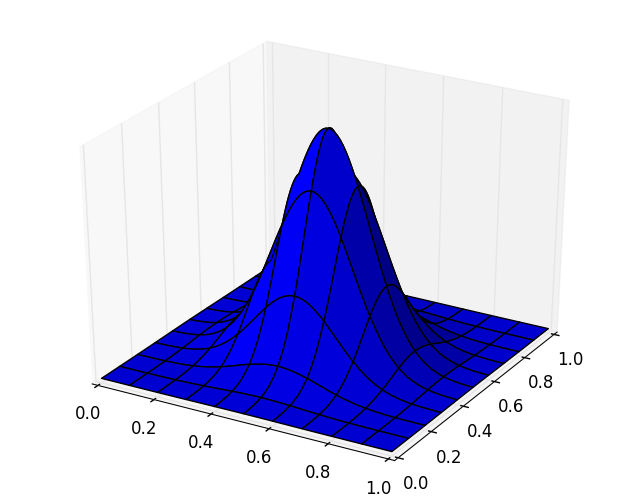
\includegraphics[width=\linewidth]{images/2dgrid_1.png}
      \vspace{-12px}
      \caption{$f(x) = \mathcal{N}(\vec{x})$}
      \endminipage
      \minipage{0.5\textwidth}
      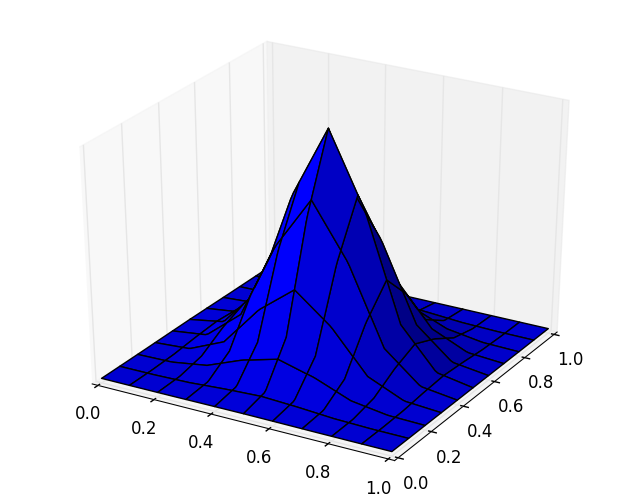
\includegraphics[width=\linewidth]{images/2dgrid_2.png}
      \vspace{-12px}
      \caption{Full grid discretization $\hat{f}_1(x_1) \cdot \hat{f}_2(x_2)$}
      \endminipage
    \end{figure}
  \end{block}
\end{frame}

\begin{frame}
  \frametitle{Full Grid Discretization}
  \topline
  \vspace{-10px}
  \begin{block}{Summary}
    \begin{itemize}
      \item Girdpoints $i \in \{1..2^l\}$ defining $\phi_i(x)$
        \vspace{5px}
      \item For \emph{each} dimension: \textbf{sum over basisfunctions} $\hat{f}(x) = \sum_i{\alpha_i \phi_i(x)}$
        \vspace{5px}
      \item For \emph{all} dimensions: \textbf{product over dimensions} $\prod{\hat{f}(x)}$
    \end{itemize}

  \end{block}
\end{frame}

%%% Local Variables:
%%% TeX-master: "slides"
%%% End:
